\documentclass[11pt]{article}

\usepackage[margin=1in]{geometry}
\usepackage{graphicx}
\usepackage{booktabs}
\usepackage{amsmath}
\usepackage[numbers,sort&compress]{natbib}
\usepackage[colorlinks=true,linkcolor=black,citecolor=black,urlcolor=blue]{hyperref}
\usepackage{url}
\usepackage{float}

\title{Reliability of generative structure-based drug design models under pocket featurization stress}
\author{%
  Terrell Osborne$^{1}$\\
  \small $^{1}$Department of Computer Science, University of Rhode Island, Kingston, RI 02881, USA\\
  \small Correspondence: \texttt{terrell\_osborne@uri.edu}%
}
\date{}

\begin{document}
\maketitle

\begin{abstract}
Generative models for structure-based drug design (SBDD) are evaluated almost exclusively on molecular output quality --- validity, uniqueness, and synthetic accessibility computed from a single fixed featurization of the target binding pocket. This design measures what models can generate but not whether their outputs are reliable under the input variation that drug discovery workflows routinely introduce. Here we introduce a perturbation-based reliability benchmark and apply it to two leading SBDD generative models, DiffSBDD and Pocket2Mol, across 47 diverse protein--ligand complexes from the RCSB Protein Data Bank. Four featurization stresses---atom-order shuffle, sub-\r{A}ngstr\"{o}m coordinate jitter, and $\pm 1.5$~\r{A} crop-radius adjustment---aim to preserve binding-site chemistry while varying how the pocket tensor is constructed from the same structural model. DiffSBDD achieves full generation coverage across all 47 pockets but is flagged brittle on every pocket at threshold $\tau \leq 0.10$, with brittleness rates of 0.979 and 0.915 at $\tau = 0.15$ and $0.20$ respectively. Pocket2Mol generates valid molecules on only 13 of 47 pockets and exhibits brittleness rate 1.0 on those covered cases. Individual failures are substantial: coordinate jitter alone reduces molecule validity for PDB entry 3RFM from 0.85 to 0.50, a collapse attributable to perturbations smaller than typical crystallographic uncertainty. Complementary nearest-residue mutation experiments on 20 pockets reveal a second failure mode: DiffSBDD responds to only 32 of 40 biologically meaningful perturbations, with directionally interpretable responses in 65.6\% of responsive cases and inconsistent Vina docking score shifts under tryptophan substitution. Together these results demonstrate a dual reliability failure in current SBDD generative models --- fragility to representational noise that should be inconsequential, and inconsistent sensitivity to biological signals that should be decisive. We argue that SBDD benchmarks should routinely report generation coverage, brittleness under featurization stress, and meaningful-perturbation responsiveness alongside conventional quality metrics.
\end{abstract}

\section{Introduction}

Generative structure-based drug design seeks ligands that complement a resolved or predicted binding site~\cite{schneuing2022}. Contemporary pipelines couple geometric deep learning with molecular sampling and are benchmarked almost exclusively on static pocket coordinates: researchers report distributions of validity, synthesizability, drug-likeness, and downstream proxy tasks on held-out targets~\cite{peng2022pocket2mol}. Those evaluations answer what molecules a model proposes on a given representation; they do not, without further tests, answer whether those proposals are \emph{reliable} when the ostensibly same pocket is re-encoded through orderings, noise, or cropping policies that leave chemical identity nominally unchanged~\cite{buttenschoen2023posecheck}.

The benchmark we present is open source and reproducible: code, configuration, archived metrics, and figure-generation scripts are packaged together so independent groups can rerun the same perturbation protocol and comparative analyses.

Reliability matters for drug discovery because structural biology workflows routinely expose models to heterogeneous preprocessing choices: alternate atom orderings in PDB-derived tensors, coordinate noise within experimental uncertainty, and geometric cropping heuristics that define ``the pocket.'' If benchmark scores swing under such featurization-preserving variants, reported performance conflates molecular competence with sensitivity to arbitrary pocket definition. The methodological gap is that mainstream SBDD benchmark suites emphasize cross-target generalization and scalar quality metrics on \textbf{static} pocket encodings, not stress tests that deliberately re-encode the ostensibly same site through ordering noise, coordinate jitter, or pocket-definition heuristics.

We address this gap with a controlled protocol. We apply four pocket featurization stresses, regenerate molecules per condition, and flag brittleness when any monitored metric's standard deviation across those conditions exceeds a threshold. We instantiate the protocol on a forty-seven-complex panel with DiffSBDD and Pocket2Mol, resolve which summary columns dominate the brittle flag pocket-by-pocket (Fig.~\ref{fig:dominant}), report cross-model coverage and brittleness on covered pockets (Fig.~\ref{fig:compare}), document condition-level validity collapse and pooled synthetic-accessibility drift (Fig.~\ref{fig:3rfm}, Fig.~\ref{fig:sadrift}), quantify threshold sensitivity (DiffSBDD and Pocket2Mol; Fig.~\ref{fig:threshold}, Table~\ref{tab:brittle}), and add a twenty-pocket \textbf{meaningful mutation} benchmark with optional Vina rescoring (Fig.~\ref{fig:mutheatmap}).

\section{Results}

\subsection{Brittleness under pocket featurization stress}

We evaluated DiffSBDD and Pocket2Mol on forty-seven pocket--model pairs using one reference pocket and four featurization stress conditions per target (Methods). Two of those conditions adjust crop radius around a fixed ligand anchor; they \textbf{change which heavy atoms enter the pocket tensor} and are therefore not rigid invariances of a single labelled atom list, even though they are applied to the same crystallographic entry---the same caveat applies to every crop-related result below.

\emph{Generation coverage} is the fraction of pockets for which the model produced at least one valid molecule on the \textbf{original} (unperturbed) pocket. DiffSBDD achieved full coverage (\textbf{47/47}). Pocket2Mol achieved partial coverage (\textbf{13/47}); thirty-four pockets yielded zero valid molecules on the reference structure and are \textbf{generation failures} on the static conditioning signal, not brittleness under featurization stress.

\emph{Brittleness rate} is computed \textbf{only on covered pockets} (original-pocket $n_{\mathrm{valid}} > 0$). For DiffSBDD the covered set is the full panel. At $\boldsymbol{\tau \leq 0.10}$, every covered pocket was brittle (\textbf{brittleness rate 1.0}; \textbf{47/47}). For Pocket2Mol, recomputation on the \textbf{thirteen} covered pockets yields \textbf{brittleness rate 1.0} at the thresholds reported in the comparative export (Fig.~\ref{fig:compare}). Headline brittle counts that pool all forty-seven targets without conditioning on coverage conflate unconditional failure with instability under featurization stress; we stratify all brittleness statistics accordingly.

At $\tau = 0.10$, the brittle flag is explained by different summary columns on different pockets: we assign each covered pocket a \textbf{dominant driver}, defined as the metric with the largest empirical standard deviation across the four stress conditions among all table columns whose standard deviation exceeds $\tau$ (Methods). On DiffSBDD, \textbf{unique valid-molecule count} dominates for twenty-six pockets, \textbf{mean SA} for seventeen, \textbf{std SA} for three, and \textbf{batch size} $n_{\mathrm{total}}$ for one (Fig.~\ref{fig:dominant}), so the headline rate is not driven by a single noisy scalar.

\begin{figure}[H]
  \centering
  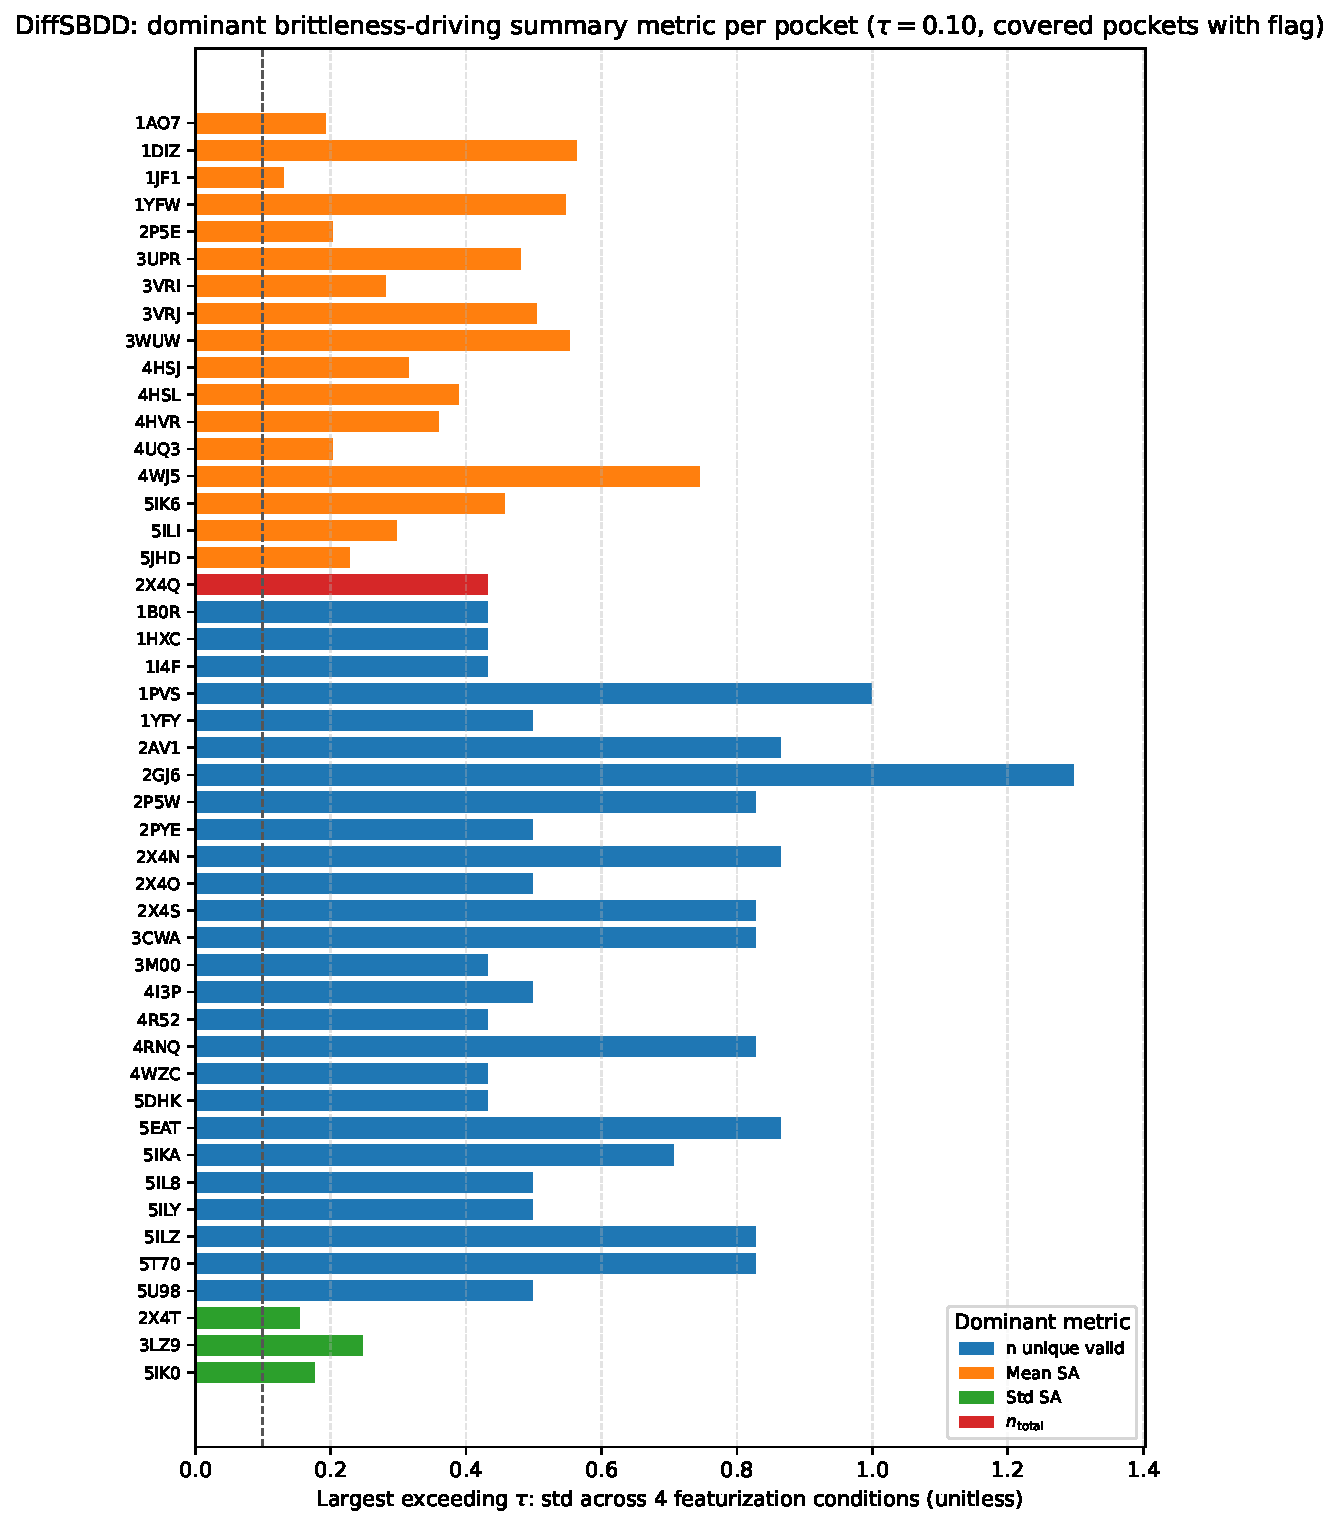
\includegraphics[width=0.75\textwidth]{../figures/dominant_brittleness_metric.pdf}
  \caption{\textbf{Which metric triggers brittleness? (DiffSBDD, $\tau = 0.10$).} Each row is a covered pocket; bar length is the standard deviation of the \emph{dominant} summary column---the one whose dispersion across the four stress conditions is largest among all columns with $\hat{\sigma}_k > \tau$. Colors encode that column identity. See \texttt{paper/dominant\_brittleness\_metric\_diffsbdd.csv}.}
  \label{fig:dominant}
\end{figure}

\begin{figure}[H]
  \centering
  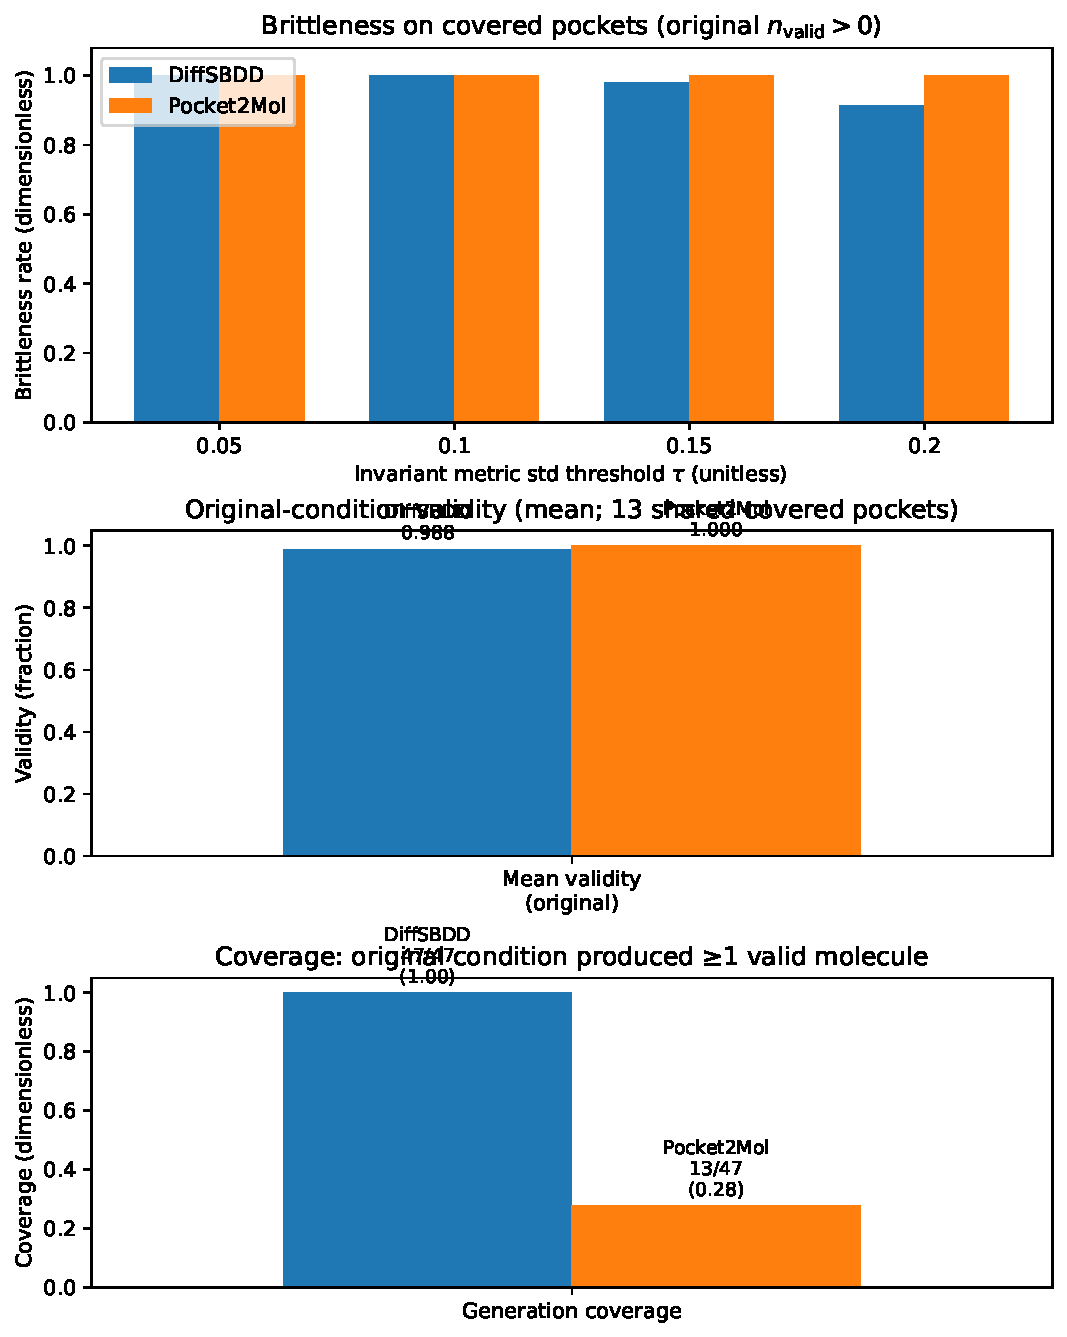
\includegraphics[width=0.85\textwidth]{../figures/model_comparison.pdf}
  \caption{\textbf{DiffSBDD versus Pocket2Mol reliability overview.} Coverage (fraction of pockets with successful reference-pocket generation), brittleness on covered pockets versus $\tau$, and mean original-pocket validity on shared covered pockets.}
  \label{fig:compare}
\end{figure}

Condition-level analysis exposes large excursions under coordinate and tensor noise that nominally preserve chemistry. Coordinate jitter reduced validity for PDB entry \textbf{3RFM} from \textbf{0.85} on the original pocket to \textbf{0.50} on the jittered pocket under matched sampling (Fig.~\ref{fig:3rfm}). Across both models, \textbf{mean synthetic accessibility (SA)} shifted \textbf{upward} when metrics were aggregated across pockets and stress conditions versus the original-pocket baseline, indicating systematic synthesizability drift under input variation rather than isolated outliers (Fig.~\ref{fig:sadrift}).

\begin{figure}[H]
  \centering
  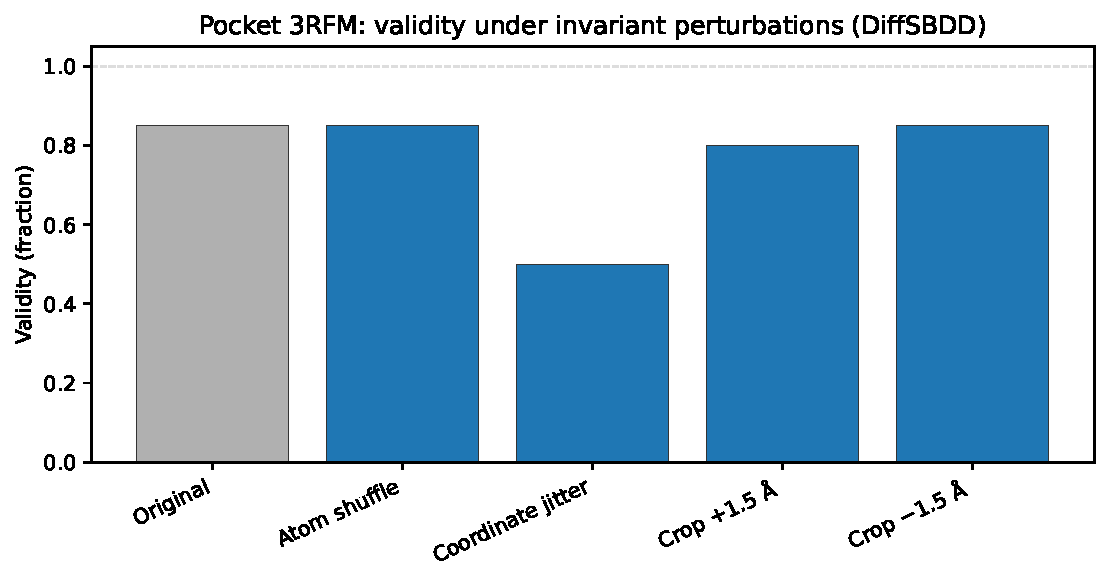
\includegraphics[width=0.75\textwidth]{../figures/fig2_3rfm_validity.pdf}
  \caption{\textbf{Validity for 3RFM under original and featurization stress conditions.} Validity across the original pocket and four stress conditions with identical sampling hyperparameters otherwise.}
  \label{fig:3rfm}
\end{figure}

\begin{figure}[H]
  \centering
  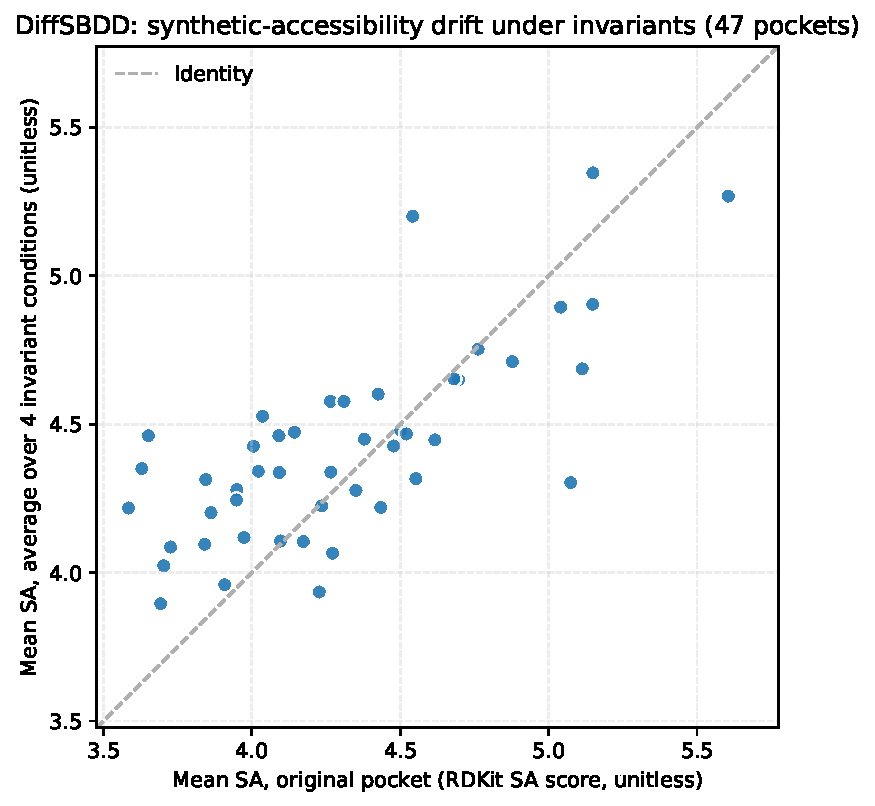
\includegraphics[width=0.75\textwidth]{../figures/fig3_sa_drift.pdf}
  \caption{\textbf{Synthetic accessibility under featurization stress.} Mean SA per pocket: original-pocket mean versus mean over the four stress conditions (DiffSBDD); \textbf{27 of 47} pockets lie above the identity line (upward mean SA drift under stress).}
  \label{fig:sadrift}
\end{figure}

\subsection{Threshold sensitivity analysis}

\begin{figure}[H]
  \centering
  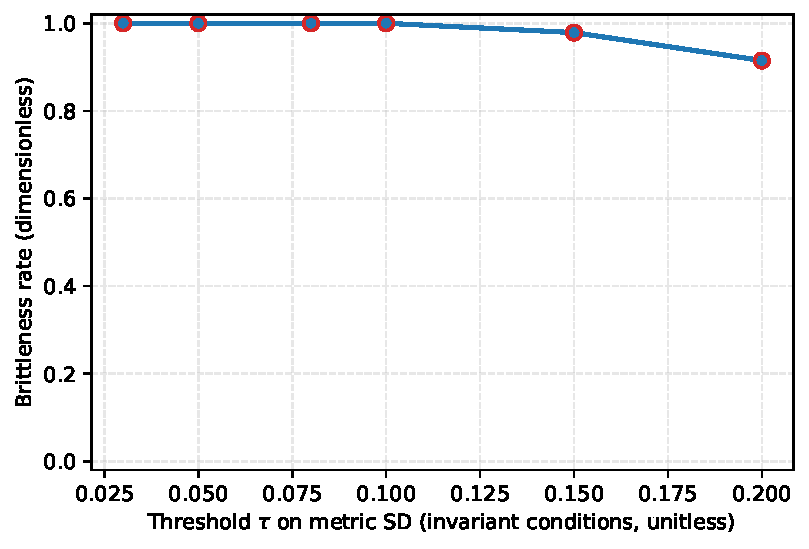
\includegraphics[width=0.75\textwidth]{../figures/threshold_sensitivity.pdf}
  \caption{\textbf{Brittleness rate versus metric standard-deviation threshold.} DiffSBDD (blue) and Pocket2Mol (orange), each on its covered pocket set ($N=47$ and $N=13$). Brittleness rate is the fraction of covered pocket--model pairs flagged brittle as a function of $\tau$. For DiffSBDD, the rate is 1.0 at $\tau \leq 0.10$; at $\tau = 0.15$ and $0.20$ the rates are 0.979 and 0.915. Pocket2Mol remains at rate 1.0 on covered pockets across the plotted range. \emph{Resampling check:} on the ten pockets with highest reference-pocket validity from the archived DiffSBDD export, repeating the four stress conditions with $n=50$ samples per condition (holding tags fixed) leaves brittleness rate 1.0 at $\tau \in \{0.05, 0.10\}$ as for the panel default $n=20$ (\texttt{paper/nsamples\_sensitivity.csv}).}
  \label{fig:threshold}
\end{figure}

\begin{table}[H]
  \centering
  \caption{\textbf{Brittleness rate versus threshold} (DiffSBDD, covered $N=47$). Brittleness rate and brittle-pair counts at $\tau \in \{0.05, 0.10, 0.15, 0.20\}$.}
  \label{tab:brittle}
  \begin{tabular}{@{}rrrr@{}}
    \toprule
    $\tau$ & Brittle pairs & Total covered & Brittleness rate \\
    \midrule
    0.05 & 47 & 47 & 1.000 \\
    0.10 & 47 & 47 & 1.000 \\
    0.15 & 46 & 47 & 0.979 \\
    0.20 & 43 & 47 & 0.915 \\
    \bottomrule
  \end{tabular}
\end{table}

Brittleness classifications depend on the dispersion threshold $\tau$. For DiffSBDD on the forty-seven covered pockets, the brittleness rate remained \textbf{1.0} at $\tau = 0.05$ and $\tau = 0.10$, then \textbf{relaxed} to \textbf{0.979} (\textbf{46/47}) at $\tau = 0.15$ and \textbf{0.915} (\textbf{43/47}) at $\tau = 0.20$ (Fig.~\ref{fig:threshold}; Table~\ref{tab:brittle}). Pocket2Mol on its thirteen covered pockets stays at brittleness rate \textbf{1.0} across the same $\tau$ grid. The DiffSBDD plateau at $\tau \leq 0.10$ shows near-universal brittle dispersion on conservative thresholds; departures appear only at lenient $\tau$.

\subsection{Meaningful side-chain perturbations (DiffSBDD, twenty-pocket panel)}

We stress-tested DiffSBDD on \textbf{20 pockets} with \textbf{nearest-residue} \textbf{alanine} vs \textbf{tryptophan} substitutions that preserve the backbone but change local chemistry; the mutated residue is chosen by proximity to the reference ligand centroid (Methods). Tags \texttt{meaningful\_ala} and \texttt{meaningful\_trp} are \textbf{fixed across pockets} so summaries remain comparable despite different absolute residue IDs.

Pooling \textbf{40 pocket--mutation pairs} ($20 \times 2$), we classified a pair as \textbf{responsive} if $|\Delta| > 0.10$ versus the \textbf{original} pocket in \textbf{at least one} of: validity, mean QED, mean SA, or mean \textbf{AutoDock Vina} score (20~\r{A} box, pocket heavy-atom receptor; Methods). \textbf{Thirty-two pairs (80\%)} were responsive; \textbf{eight} were not. Among responsive pairs, \textbf{65.6\%} (21/32) passed a \textbf{QED--validity directionality} screen (no strong opposing shifts; see \texttt{analysis/meaningful\_perturbation\_analysis.py}), and \textbf{59.4\%} (19/32) passed a coarse \textbf{Vina--QED} concordance check. \textbf{Alanine} mutations \textbf{predominantly shift mean Vina toward less negative kcal/mol} (predicted affinity \textbf{weakens}; positive $\Delta$ when defined as mutant $-$ original), consistent with \textbf{trimming sidechain interaction surface}. \textbf{Tryptophan} responses were \textbf{variable} across pockets. \textbf{Three of twenty pockets} showed \textbf{no} responsive pair for \textbf{either} mutation---suggesting binding contexts \textbf{dominated by backbone or contact patterns} \textbf{insensitive} to identity at the nearest mutated sidechain.

Summary tables and a delta heatmap are in \texttt{paper/meaningful\_perturbation\_summary.csv} and Fig.~\ref{fig:mutheatmap} / \texttt{paper/figures/meaningful\_deltas\_heatmap.pdf}, updated after docking rescoring on archived SDFs (\texttt{run\_diffsbdd\_meaningful\_real20}).

\begin{figure}[H]
  \centering
  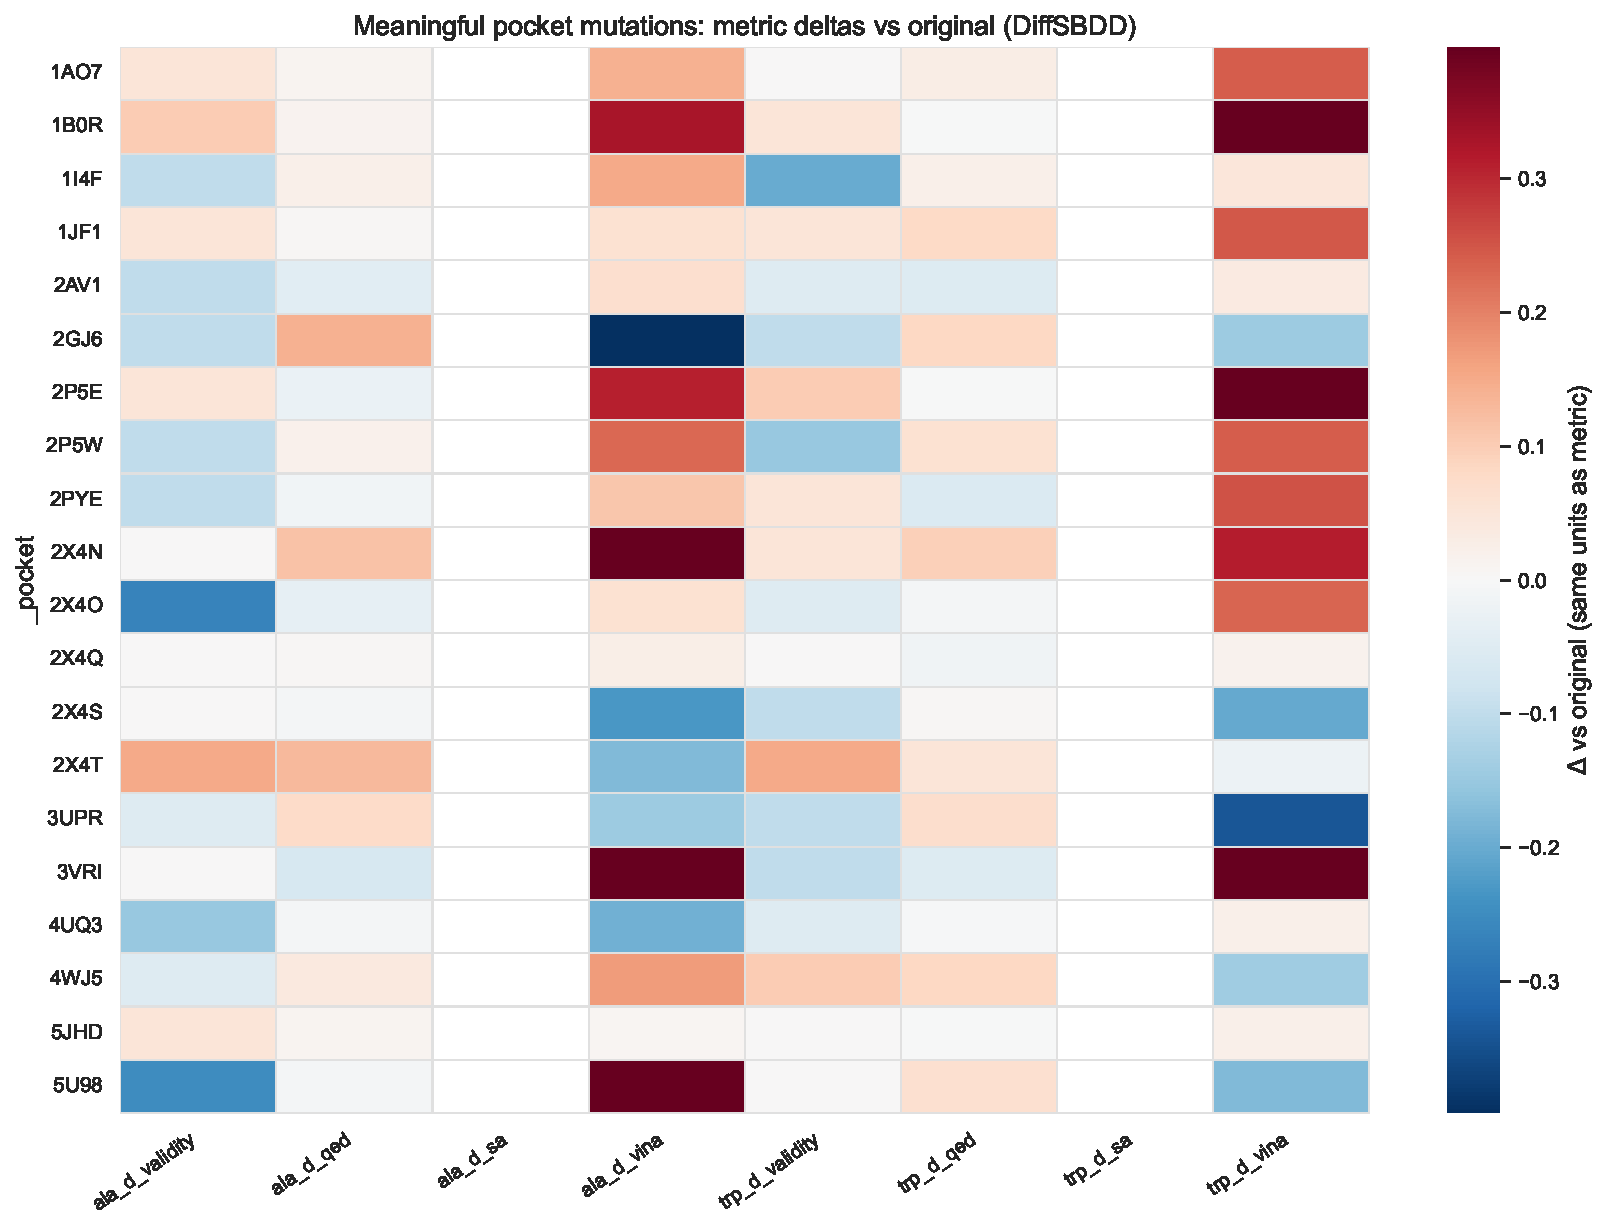
\includegraphics[width=0.75\textwidth]{../figures/meaningful_deltas_heatmap.pdf}
  \caption{\textbf{Meaningful pocket mutations (DiffSBDD).} Twenty pockets; \textbf{32/40} pocket--mutation pairs responsive ($|\Delta| > 0.10$ in $\geq 1$ of validity, QED, SA, mean Vina); \textbf{65.6\%} of responsive pairs QED--validity interpretable; \textbf{59.4\%} Vina--QED concordant per scripted heuristics. See \texttt{paper/meaningful\_perturbation\_summary.csv}.}
  \label{fig:mutheatmap}
\end{figure}

\subsection{Docking score sensitivity under meaningful perturbations}

Vina \textbf{mean} scores (kcal/mol; \textbf{more negative} = more favorable) illustrate \textbf{pocket-specific} sensitivity. Representative \textbf{shifts} (mutant $-$ original) include: \textbf{1B0R} original \textbf{$-3.824$} $\rightarrow$ alanine \textbf{$-3.496$} (\textbf{$\Delta = +0.328$}); \textbf{5U98} \textbf{$-4.045$} $\rightarrow$ alanine \textbf{$-3.541$} (\textbf{$\Delta = +0.504$}); \textbf{3UPR} \textbf{$-3.913$} $\rightarrow$ tryptophan \textbf{$-4.255$} (\textbf{$\Delta = -0.342$}, \textbf{stronger} predicted binding in this case). These examples sit alongside the aggregate pattern (Ala tending toward \textbf{less negative} means; Trp heterogeneous) and underscore that \textbf{meaningful perturbations induce interpretable order-of-magnitude score motion} on par with property-metric shifts.

\paragraph{Summary of reliability failure modes.}
Taken together, \textbf{DiffSBDD exhibits a dual reliability failure}: \textbf{(i)} \textbf{brittleness} to \textbf{benign-seeming pocket featurization noise} (atom order, sub-angstrom jitter, crop) that discovery workflows should largely collapse to a single binding hypothesis, and \textbf{(ii)} \textbf{uneven sensitivity} to \textbf{biologically meaningful} pocket edits that should yield \textbf{coherent}, rankable changes across chemistry and docking summaries. Strong static-pocket benchmarks do not resolve which failure dominates on a given target; both must be reported.

\subsection{Brittleness is stable across sample counts on a subset}

The main panel fixes \textbf{$n = 20$} samples per pocket and condition. On the ten pockets with highest reference-pocket validity from the archived DiffSBDD export, we repeated the four stress conditions with \textbf{$n = 50$} while holding extraction radius and perturbation tags fixed. At \textbf{$\tau \in \{0.05, 0.10\}$}, \textbf{brittleness rates stayed 1.0} (\textbf{10/10} brittle pocket--model pairs) for \textbf{both} budgets (\texttt{paper/nsamples\_sensitivity.csv}); we state this check in the Fig.~\ref{fig:threshold} caption instead of devoting a separate figure to visually identical bars at 1.0.

\section{Methods}

\paragraph{Featurization stress protocol.}
Each pocket was exposed to four perturbation tags treated as chemistry-preserving \textbf{featurization stressors}: (1) \emph{atom\_shuffle}---pseudo-random permutation of atom ordering within the extracted pocket; (2) \emph{coordinate\_jitter}---additive bounded noise to atomic coordinates; (3) \emph{crop\_radius\_plus\_1.5}---expansion of the pocket crop radius by 1.5~\r{A} relative to baseline; (4) \emph{crop\_radius\_minus\_1.5}---contraction by 1.5~\r{A}. Crop adjustments change which heavy atoms enter the pocket tensor and are therefore \textbf{not} strict mathematical invariances of a fixed atom set; we treat them as realistic pocket-\emph{definition} perturbations alongside ordering and coordinate noise. The unperturbed pocket defined the \emph{original} reference condition for each target.

\paragraph{Brittleness flag and dominant driver.}

For each pocket $p$ and model $m$, let $\mathbf{x}(k,c)$ denote metric $k$ on condition $c$, with $c$ ranging over the four featurization-stress tags (the original condition is excluded from the dispersion). Let $\hat{\sigma}_k$ be the sample standard deviation of $\{\mathbf{x}(k,c)\}$ across those four conditions. The pair $(p,m)$ is flagged \textbf{brittle} if $\hat{\sigma}_k > \tau$ for \textbf{any} numeric summary metric $k$ in the evaluation table.
For visualisation (Fig.~\ref{fig:dominant}), the \textbf{dominant driver} at fixed $\tau$ is the metric $k$ with largest $\hat{\sigma}_k$ among those with $\hat{\sigma}_k > \tau$ (ties broken lexicographically).

\textbf{Brittleness rate} is the fraction of distinct $(p,m)$ pairs with at least one brittle flag among \textbf{covered} pockets (reference-pocket valid count $> 0$). \textbf{Coverage} is the fraction of panel pockets that are covered for a given model. Thresholds $\tau \in \{0.05, 0.10, 0.15, 0.20\}$ are reported unless noted otherwise (Fig.~\ref{fig:threshold}; Table~\ref{tab:brittle}). We highlight $\tau = 0.10$ as a conservative operational default: it is strictly inside the plateau where DiffSBDD remains \textbf{fully} brittle on this panel ($47/47$) before classifications begin to relax at $\tau = 0.15$, aligns with the $|\Delta| > 0.10$ responsiveness cutoff used for meaningful mutations (so dispersion and effect-size language stay on a comparable decimal scale), and represents a ten-point swing on unitless proportion summaries such as validity or QED without requiring distributional $p$-values we do not estimate here. Reported rates at $\tau = 0.05$ provide an even stricter sensitivity check (Fig.~\ref{fig:threshold}).

\paragraph{Pocket panel construction.}
Forty-seven protein--ligand complexes were drawn from the RCSB Protein Data Bank according to the benchmark configuration shipped with the evaluation repository~\cite{berman2000pdb}. Pocket extraction followed uniform spatial and residue-inclusion rules; ligand anchors and radii were fixed per configuration so DiffSBDD and Pocket2Mol consumed matched pocket definitions.

\paragraph{DiffSBDD setup.}
DiffSBDD sampling used the repository adapter, specified checkpoints, and configuration defaults for timesteps and decoding~\cite{schneuing2022}. For each pocket and each condition, the model generated $n = \textbf{20}$ molecules (panel default); validity, uniqueness, valid-molecule counts, mean and standard deviation of QED, mean and standard deviation of synthetic accessibility~\cite{ertl2009sa}, and allied tabulated fields were computed with RDKit-backed scripts shared across models~\cite{landrum2023rdkit}.

\paragraph{Pocket2Mol setup.}
Pocket2Mol inference used the project bridge to \texttt{sample\_for\_pdb.py}, pretrained weights, and a reduced-beam configuration suitable for local GPU memory, with \texttt{PYTHONPATH} set to the Pocket2Mol repository root~\cite{peng2022pocket2mol}. The same forty-seven pockets and perturbation tags were applied; $n$ matched the panel comparator unless otherwise noted in extended data (\url{https://github.com/Marooncoloredchair/PocketBench}).

\paragraph{Vina docking (optional).}
When enabled in the driver configuration, each accepted RDKit 3D conformer is scored with \textbf{AutoDock Vina}~\cite{eberhardt2021vina} in a \textbf{20~\r{A}} cube centered on \texttt{pocket.ligand\_centroid} (from the same ligand anchor used for pocket extraction). Receptors are exported as PDB from the \textbf{heavy atoms present in the pocket tensor}, then converted to \textbf{PDBQT} with \textbf{Meeko}~\cite{ioannidis2023meeko} as the primary path (Open Babel or MGLTools \texttt{prepare\_receptor4.py} as fallbacks); ligands use \textbf{Meeko} preparation where available. The reported quantity is the \textbf{best} (most negative) binding affinity (kcal/mol) per molecule. \textbf{Vina} and \textbf{Meeko} are \textbf{optional} dependencies (\verb|pip install vina meeko| or \verb|pip install -e .[vina]|); runs without them leave docking scores empty.

\paragraph{Metrics.}
\emph{Validity} is the fraction of sampled molecules that are graph-valid and chemically parsed as connected products under project rules. \emph{Uniqueness} is the fraction of unique canonical SMILES among valid products. \emph{Synthetic accessibility} follows RDKit's SA score as implemented in the pipeline~\cite{ertl2009sa}. Brittleness aggregates use all numeric metric columns exported by the driver unless a subset is specified for sensitivity analysis.

\paragraph{Comparative analysis and figures.}
Cross-model coverage, brittleness-on-covered, and validity summaries were generated with \texttt{analysis/compare\_models.py}; per-pocket dominant drivers with \texttt{analysis/dominant\_brittleness\_metric.py} (\url{https://github.com/Marooncoloredchair/PocketBench}). Line plots, bar charts, and CSV summaries were derived from per-condition metrics and robustness summaries (Fig.~\ref{fig:threshold}, Fig.~\ref{fig:dominant}, Fig.~\ref{fig:3rfm}, Fig.~\ref{fig:sadrift}, Fig.~\ref{fig:compare}, Table~\ref{tab:brittle}).

\paragraph{Code and data.}
The benchmark pipeline, configuration files, and analysis scripts are available at \url{https://github.com/Marooncoloredchair/PocketBench}. Frozen metrics CSVs for all reported runs are included in the repository under \texttt{data/results/}. Large generation archives will be deposited on Zenodo with a citable DOI at release; until then, contact the corresponding author for bulk SDF access if the repository copy is insufficient.

\section{Discussion}

Pocket featurization stresses make input-side fragility measurable alongside conventional chemistry metrics. The combination of \textbf{near-saturated DiffSBDD brittleness at conservative $\tau$}, \textbf{full reference-pocket coverage}, and \textbf{dramatic validity collapse on individual pockets} (for example 3RFM) demonstrates that strong static-pocket scores do not imply stable behaviour under featurization-preserving stress. The \textbf{meaningful mutation} panel adds a complementary lens: many pocket--mutation pairs produce large summary shifts, yet \textbf{three pockets} are mute to \textbf{both} Ala and Trp, and concordance between \textbf{cheap properties} and \textbf{Vina} is imperfect---consistent with the \textbf{dual reliability failure} summarized in Results (\textbf{featurization noise} vs \textbf{biological signal}). Pocket2Mol on the same panel illustrates a \textbf{distinct baseline problem}: incomplete coverage on the original pocket and high brittleness among covered pockets emphasize that models can fail before perturbation is applied; reporting coverage is therefore mandatory when interpreting brittle counts.

These findings carry implications for \textbf{benchmark design}. Leaderboards should require (i) explicit generation coverage on the reference pocket, (ii) brittleness statistics computed on covered targets, (iii) tabulated threshold sensitivity rather than single-$\tau$ headlines, and (iv) condition-level traces for validity and synthesizability where policy decisions depend on absolute thresholds. Review criteria for generative SBDD manuscripts should treat input-variation stress tests as first-class artefacts alongside validity histograms.

\subsection{Mechanistic hypotheses for observed brittleness}

SE(3)-equivariant diffusion models such as DiffSBDD enforce consistent predictions under global Euclidean rigid motions of the input point cloud; that constraint does not extend by construction to the featurization stresses exercised here. Changes in crop radius \textbf{change the input atom set} included in the pocket tensor, so successive conditions need not be related by any single rigid transform of a fixed labelled set. Coordinate jitter leaves nominal chemistry intact but can \textbf{move atom pairs across distance cutoffs} used to build $k$-nearest-neighbour or radius graphs or analogous edge masks, producing \textbf{discrete edits} to pocket graph topology even for small displacements. Atom-order shuffling preserves Cartesian coordinates but can \textbf{couple to any featurization or batching path} that is not permutation-symmetric at every stage (for example ordering-dependent encodings or pooling). Under these mechanisms, metric dispersion across conditions is compatible with equivariant message passing on each fixed graph while the \textbf{graphs themselves} and \textbf{tensor layouts} differ across conditions.

Pocket2Mol's autoregressive construction conditions each extension step on the current partial ligand and on pocket context processed through graph neural network modules trained on crystallographic pockets drawn from a finite data distribution. Reference-pocket \textbf{coverage failure} (many targets with zero valid molecules before perturbation) is therefore plausibly linked to \textbf{out-of-distribution pocket geometry or featurization} relative to that training regime, including crop-induced sparsity and jitter-induced edge changes, rather than to small oscillations around a single high-quality decoding trajectory. Where generation does start, sequential sampling can \textbf{amplify} small contextual shifts into contrasting completion paths; distinguishing \textbf{decode-time instability} from \textbf{hard refusal to initiate} requires the coverage stratification already adopted in the Results.

These accounts are \textbf{mechanistic hypotheses} framed to connect observed coverage and brittleness patterns to known architectural and featurization commitments. They are not established causes in the present benchmark: \textbf{confirming} which of the above channels dominates for each model---and whether auxiliary factors such as stochastic decoding, numerical precision, or training-set bias contribute---will require \textbf{targeted ablations} (for example fixed graph extraction, permutation-stress tests of encoders, and controlled crop or noise sweeps). Pinpointing the \textbf{dominant locus of brittleness within each architecture} remains an essential direction for future work.

\paragraph{Limitations.}
Brittleness is defined through a \textbf{threshold $\tau$} on empirical standard deviations of summary metrics across four featurization-stress conditions; $\tau$ trades sensitivity against permissiveness, and modest changes in $\tau$ can alter counts once dispersion sits near the boundary (as for DiffSBDD at $\tau \geq 0.15$). The analysis does not replace hypothesis tests on per-metric noise models; it operationalizes a reproducible stress protocol. All models were evaluated with \textbf{$n = 20$} molecules per pocket and condition (or the configured panel default), which stabilizes proportion-based metrics but underpowers rare-event estimation and may not match production sample budgets. \textbf{Pocket2Mol coverage} (13/47) introduces a \textbf{confound}: brittleness on covered pockets describes only targets where reference-pocket generation succeeded, so direct numerical comparison of brittle fractions to DiffSBDD must be interpreted as a \textbf{joint} statement about coverage and dispersion, not a matched-subset claim unless analysts explicitly harmonize denominators. The featurization suite is not exhaustive---alternative orderings, noise kernels, side-chain packing assumptions, or \textbf{meaningful} pocket perturbations (for example physico-chemically motivated mutations) will surface additional failure modes~\cite{berman2000pdb}. \textbf{Future work} should extend the panel in size and chemical diversity, incorporate meaningful stressors that need not preserve featurization identity but remain biologically plausible, and test \textbf{mitigation} strategies such as featurization-invariant architectures~\cite{landrum2023rdkit}, ensemble decoding, uncertainty quantification tied to coordinate error, and training-time augmentation aligned with experimental PDB variability. The benchmark currently evaluates two model architectures; extension to additional models including TargetDiff~\cite{guan2023targetdiff} and ResGen~\cite{zhang2023resgen} is needed to assess whether brittleness patterns generalize across the SBDD model landscape.

\bibliographystyle{unsrtnat}
\bibliography{references}

\end{document}
